\chapter{Contur Overview}
\label{chapterlabel2}

\section{Contur and the Standard Model}
The standard model (SM) of particle physics is the name for the collective of quantum field theories that successfully describe three of the four fundamental forces of nature\footnote{The forces successfully described are the electromagnetic force, the weak force and the strong force, while a quantum theory of gravity still eludes us} and the observable matter content of the universe\footnote{For further details into the theory see \cite{sm_text_1} or \cite{sm_text_2}}. The success of the SM is evidenced by the generally strong agreement between SM predictions and experimental data\footnote{For example the observation of the Higgs Boson\cite{sm_prove}}. Despite this success there is a widespread view that the SM is not the complete picture. This viewpoint arises from the inability of the SM to accommodate gravity or provide any insight into postulated quantities like dark matter\footnote{Dark matter is hypothetical form of matter postulated to explain discrepancies between observed astrophysical motion and what we would expect based off the gravitational equation of motion in general relativity} and dark energy\footnote{Dark energy is a hypothetical force postulated to explain the observed expansion of the universe}. As a result the task of the developing new fundamental theories in physics that extend the SM, which we will term Beyond Standard Model theories, is an active area of research.

\textbf{Contur}(Constraints On New Theories Using Rivet) has been developed to aid the search for new BSM theories. The approach aims to leverage the large amount of experimental data produced at the Large Hadron Collider to set constraints on the type of BSM theories which are possible. This is done by considering experimental results which have already been shown to agree with SM expectations. The \textbf{Contur} procedure then asks  the question for a given completely specified BSM theory, where by completely specified we mean that the values of all free parameters have been set, \say{at what significance do existing measurements which agree with the SM already exclude this BSM}. 

The approach thus checks the consistency of predictions of the BSM theory against experimental results that have already been shown to align well with SM predictions. The idea being if the BSM theory is inconsistent with the experimental data and fails to predict processes accurately that are already well understood within the SM, then the BSM with parameter values we specified is not viable. Through running \textbf{Contur} for the BSM theory for multiple different free parameter values we can rule out parameter values which are inconsistent with realised data or potentially even rule out the whole BSM theory if there are no values for the free parameters of the BSM theory that produce consistent predictions.

\section{Input Data}\label{data}

\textbf{Contur's} consistency checks compare simulated data from a new BSM theory against realised experimental data. We will now outline in greater detail how these two main sources of data are sourced.

\subsection{Simulated BSM Data}

At first sight the need to produce a large amount of simulated results for a BSM theory for a \textbf{Contur} run would seemingly jeopardise the desire that \textbf{Contur} to be a relatively quick and easy way to check the consistency of the BSM theory with realised data. If for every BSM theory run on \textbf{Contur} scripts of bespoke ancillary code was necessary to produce simulations of the BSM theory something like the \textbf{Contur} procedure would likely not be practicable. 

Fortunately there exists mature packages in the particle physics community specifically devoted to the tasks of simulating particle collision events. These packages are sufficiently flexible that they can be used to simulate both SM events and a wide array of BSM events. A large part of this flexibility comes from the Universal FeynRules Output (UFO)\cite{ufo}, which allows the encoding of the Feymann diagram information of a process in a standard form which can then be passed to an event generator which can use Monte Carlo methods to simulate the event in question.

\textbf{Contur} is event generator agnostic in the sense that any generator that can produce simulations with data in the required final format could be used. Yet, despite this, the main event generator currently used by \textbf{Contur} is \textbf{Herwig}\cite{herwig} and the default assumption within the current set up is that the user generates BSM data with \textbf{Herwig}. For a fully specified BSM theory \textbf{Herwig} will generate events for a range of scenarios, with the output of these simulations being a collection of histograms\footnote{See figure \ref{fig:example_histogram} below for an example of a histogram used}, where any given bucket in these plots is the number of signal events which were counted in that bucket for the BSM theory. All of this output is stored in a single \textbf{YODA} file\cite{yoda}, this \textbf{YODA} file contains all the simulation data required to run \textbf{Contur} for a fully specified BSM theory.

\begin{figure}[H]
\centering
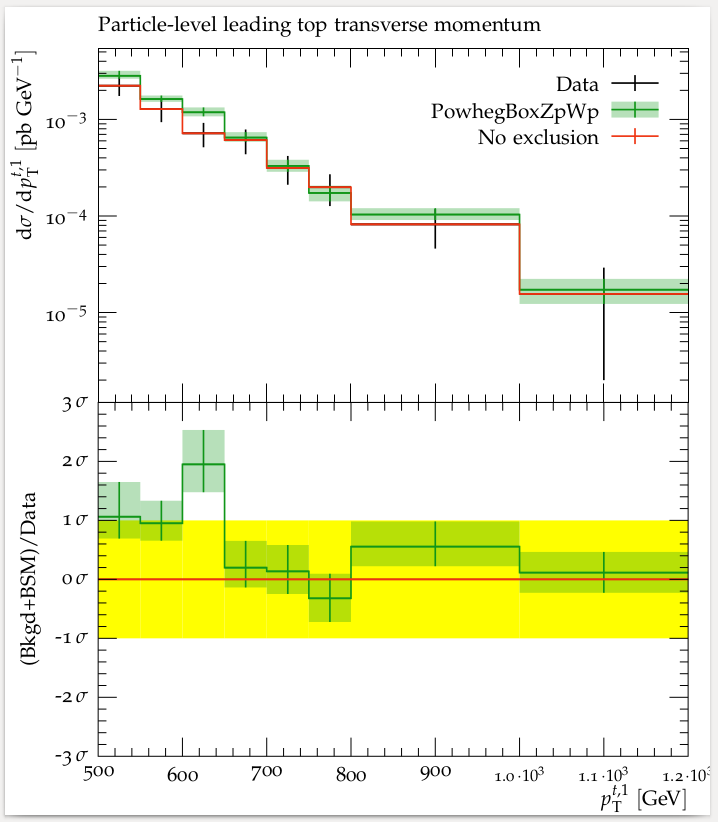
\includegraphics[scale=0.3]{plots/example_histogram.png}
\caption{Example of histogram used in \textbf{Contur}}
\label{fig:example_histogram}
\end{figure}

Recall that we previously defined a fully specified BSM theory to be the BSM with all free parameters given a single value. So running \textbf{Contur} on one fully specified BSM will only check the consistency of the BSM for the parameter values we have specified, different parameter values for the BSM will possible give different signal events changing the output. Thus for any given BSM it is likely to be the case that we want to produce multiple \textbf{YODA} files containing simulated signal events for the BSM using different parameter values across \textbf{YODA} files. 

\textbf{Contur} has tools to create a collection of such \textbf{YODA} files which is termed a grid. These tools sit within \textbf{Contur's} batch process capabilities\footnote{See Chapter 4 of the \textbf{Contur} User Manuel\cite{contur_manuel} for further details}. It is easiest to understand this process if we think of a simple example if we have a BSM theory with just two free parameters with values that can range from $1$ to $10$\footnote{For simplicity take the parameters to be dimensionless}, from this \textbf{Contur} batch can create a grid a $10\times 10$ grid of $100$ \textbf{YODA} files\footnote{\textbf{YODA} file one will be when both parameters have values 1, \textbf{YODA} file two the first parameter will have value 1, the second value 2 etc....}. We can then pass this grid to \textbf{Contur} and run a consistency check for each point on the grid, this is an example of a \textbf{Contur} grid run. The grid run is the main area of \textbf{Contur} we will later focus on in our optimisation efforts.

\subsection{Experimental Data}

\textbf{Contur} sources particle level experimental measurements from the \textbf{Rivet}\cite{Rivet} library. These particle level measurements can then be directly compared with the particle level signal effects simulated by the BSM. Carrying out the comparison at particle level ensures that the results being compared do not contain theory dependent extrapolations within them, making the \textbf{Contur} constraints arrived at independent of theoretical assumptions. 

The interface with \textbf{Rivet} is built into \textbf{Contur}, so the user does not need to provide any \textbf{Rivet} input when initiating a \textbf{Contur} run. Instead from experiments simulated in the BSM data passed in the \textbf{YODA} file \textbf{Contur} can source the appropriate experimental data from \textbf{Rivet}. In addition to realised results for experiments, simulated SM expectations can also be sourced from \textbf{Rivet}. These simulated SM expectations are created in the same way as the BSM simulations discussed in the previous subsection and stored in \textbf{YODA} files that can be accessed via \textbf{Rivet}. In its default run \textbf{Contur} does not make use of SM expectations, however there exists on optional theory run in \textbf{Contur} which we will discuss in the next section which makes use of SM expectations.

\section{Calculating Likelihoods}\label{calculate_likelihood}

The final output of a \textbf{Contur} run on a single \textbf{YODA} file is a single $CL_s$ exclusion limit, given in the form of the CL(s) technique\cite{cls}. This exclusion limit is an expression of our confidence that a fully specified BSM theory produces signal events inconsistent with understood SM processes.  The calculation of these exclusion limits is the core of the \textbf{Contur} procedure, we will now give a high level overview of the steps involved in this calculation, let us start with the default \textbf{Contur} run on a single \textbf{YODA} file.

The $CL_s$ exclusion limit is defined to be a ratio of p-values,
$$ CL_s: = \frac{CL_{s+b}}{CL_{b}} = \frac{p_{s+b}}{1- p_{b}}, $$
where in the above $p_{s+b}$ is defined as the p-value for the signal plus the background event and $p_{b}$ is the p-value just for the background event. For each histogram \textbf{Contur} computes one $CL_{s}$ by either taking the maximum $CL_{s}$ out of all the bins that compose the histogram or if correlation information between the bins exists using this to compute a single $CL_s$ for the histogram. For any given bin in a histogram, for the default \textbf{Contur} run $p_b$ will always be a half, because we are just comparing the background data with itself, so $p_{s+b}$ will compute the quantity of interest, namely how well the signal count for the BSM approach aligns with the realised count. The below code snippet shows a simplified example of the  flow of the code for the $CL_s$ calculation, the calculation takes place within the \classname{likelihood} class within \textbf{Contur}.

\begin{code}
\captionof{listing}{Compute CLs For Histogram}
\label{code:histo}
\begin{minted}{python}

def EvaluateHistogram(Histogram):
    if Histogram has correlation and (build correlation =True)
          return Likelihood(Histogram)
    else:
          return max(Likelihood(Histogram.bins))
\end{minted}
\end{code}

After computing a $CL_{s}$ for each histogram the next step is to bucket the histograms into statistically independent pools. In \textbf{Contur} a pool is combination of the final particle state, the experiment and the beam energy of the experiment, each of the three chosen so that their combination is statistical independent. Histograms that share these three properties are grouped into the same pool. \textbf{Contur} then takes the histogram with the maximum $CL_s$ in each pool. A snippet of example code used to carry out this process for a single pool is given below

\begin{code}
\captionof{listing}{Sort Likelihood blocks into pools}
\label{code:pools}
\begin{minted}{python}

def EvaluatePool(Pool):
    scores = [] #empty list for results
    if Histogram in pool:
       scores.append(EvaluateHistogram(Histogram))
    return Histogram with max(scores)
\end{minted}
\end{code}

Finally \textbf{Contur} takes the histograms from each pool and combines into a single histogram to calculate a final $CL_s$ for the \textbf{YODA} file. In combining histograms like this \textbf{Contur} assumes each of the pools to be statistical independent, which they are by construction. A simplified example of the code to perform this step is given by

\begin{code}
\captionof{listing}{Build Full Likelihood}
\label{code:full_likelihood}
\begin{minted}{python}

def BuildFullLikelihood():
      tests = []
      for Pool in ConturPools:
            tests.append(EvaliatePool(Pool))
       return Likelihood(tests)
\end{minted}
\end{code}

The main alternative run option also available in \textbf{Contur} is a theory run. In the theory run when computing the background p-value $p_b$, instead of just trivially comparing the data with itself, the SM expectations are used. So the theory \textbf{Contur} run provides more of a relative measure of which of the SM expectations or BSM expectations are in better agreement with the realised data.

As already highlighted the most common way \textbf{Contur} is used in practice is on a grid of \textbf{YODA} files as opposed to just a single file. The \textbf{Contur} grid run is not fundamentally different from the single \textbf{YODA} run, for the grid run \textbf{Contur} runs iteratively through all the \textbf{YODA} files in the grid, at each iteration calculating a single final $CL_{s}$ for the \textbf{YODA} file at that point. So the final output of the \textbf{Contur} grid run is a $CL_{s}$ value for each point on the grid. This grid of $CL_{s}$ values output can be presented as a heat map, an example of which can be seen in figure \ref{fig:example_heatmap} below.


\begin{figure}[H]
\centering
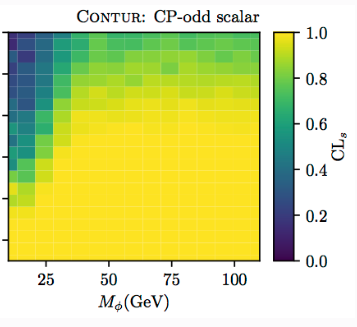
\includegraphics[scale=1]{plots/example_heatmap.png}
\caption{Example of heat map from grid run}
\label{fig:example_heatmap}
\end{figure}
